\chapter{Getting around}
\label{ch:windows}

\begin{figure}[H]
  \centering
  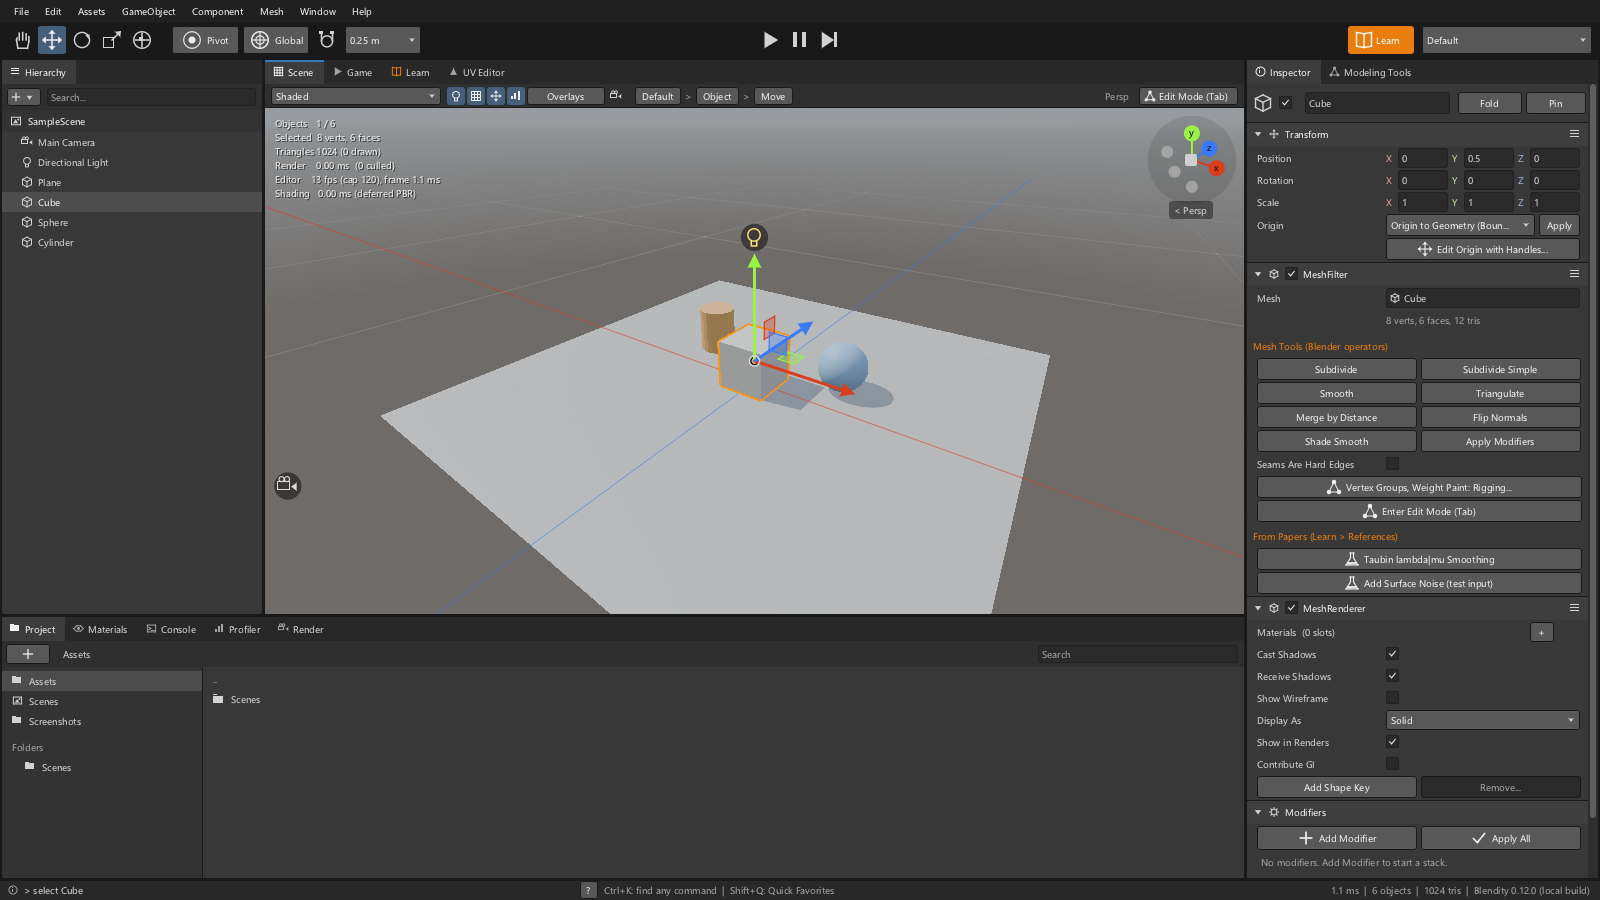
\includegraphics[width=\textwidth, alt={The Default layout of the Blendity editor: Hierarchy, Scene view, Inspector and Modeling Tools, Project and Console; the toolbar's tools, pivot, space and snap increment; Play, Pause and Step; the Learn button and the Layout dropdown at the top right.}]{editor-default.png}
  \caption{The Default layout: Hierarchy, Scene view, Inspector and Modeling Tools, Project and Console; the toolbar's
  tools, pivot, space and snap increment; Play, Pause and Step; the Learn button and the Layout dropdown at the top right.}
  \label{fig:default}
\end{figure}

\section{The windows}
\textbf{Scene} is the 3D view you edit in; \textbf{Game} shows what the active camera sees; \textbf{Hierarchy} is the
objects as a tree; \textbf{Inspector} the selected object's components; \textbf{Project} the files in \code{Assets};
\textbf{Console} the messages and a command line. Under \menu{Window} are the UV Editor, Render, Materials, Textures,
Modeling Tools, Lighting, Rigging, Animation, Sequencer, Live Link, Editing, History, Profiler, Draw, Layers, Board,
Avatar, My Tools and Learn windows. Drag a tab onto another tab bar to group it, onto a panel's edge to split it, out
past the editor's edge for a window of its own on any display; middle-click a tab to close it; right-click it for more.

\begin{fromnote}{Coming from Unity}
These are Unity's windows under Unity's names, docked the same way. \textbf{Modeling Tools} is the window Unity does
not have: every modeling, sculpting, painting and drawing tool lives there (and in the \menu{Mesh} menu), grouped by
stage.
\end{fromnote}
\begin{fromnote}{Coming from Blender}
Scene view = 3D Viewport; Hierarchy = Outliner; Inspector = Properties editor (modifiers and materials are there too);
Project = File / Asset Browser; Console = Info editor; the Layout dropdown = Workspaces. Areas split by dragging an edge
as in Blender; tabs dock as in Unity.
\end{fromnote}

\section{Layouts for each stage}
The \ui{Layout} dropdown (top right) arranges the windows for a stage of the work and shows that stage's tools and tabs
first, so the editor never feels like every tool at once. Nothing is ever gone: hidden tools still answer their keys and
the palette, \menu{Window > Layouts > Show All Tools} shows everything, and \ui{Save Layout\ldots} keeps your own.

\begin{center}
\begin{tabularx}{\textwidth}{lXX}
\toprule
Layout & Windows & Tools shown \\
\midrule
Default & everything & everything \\
Reference \& Planning & Scene, Game, Project, Board & create, reference images, cameras \\
Blocking Out & Scene, Modeling Tools & primitives, drawing, snapping \\
Modeling \& Topology & Scene, Modeling Tools & Edit Mode, checks, curves and lattices \\
UV Unwrapping & Scene beside the UV Editor & Edit Mode, UVs \\
Texturing \& Materials & Scene, Game, Materials, Textures & materials, textures, baking \\
Texturing, Stylized & Scene, Textures / Modeling Tools & surfaces, paint; strokes, scatter, sky \\
Lighting \& Rendering & Scene, Game, Lighting, Render & lights, cameras, bakes \\
Editing & Editing, Render & developing a render \\
Rigging; Skinning \& Weight Painting & Scene, Game, Rigging & bones, skins, IK, deformers; weights \\
Animation & Scene, Game, Animation along the bottom & animation, rigging, puppet posing \\
Drawing; Drawing with References & Draw, Layers, (Board) & the pen's pad, its layers, the board \\
Learning & Learn beside the Scene view & everything \\
\bottomrule
\end{tabularx}
\end{center}

In one area, Materials, Textures and Lighting fold into one \ui{Shading} tab with a row of the three under it (Rigging
\& Animation and Tools fold the same way; \ui{Fold Groups} in the tab menu turns it off). A tab strip whose labels don't
fit shows the inactive tabs as icons, then lists the rest under $\gg$; the stage's hidden tabs sit under $+N$. The
Scene view's bar reads \emph{Layout $>$ Mode $>$ Tool}, each part a dropdown.

\begin{figure}[H]
  \centering
  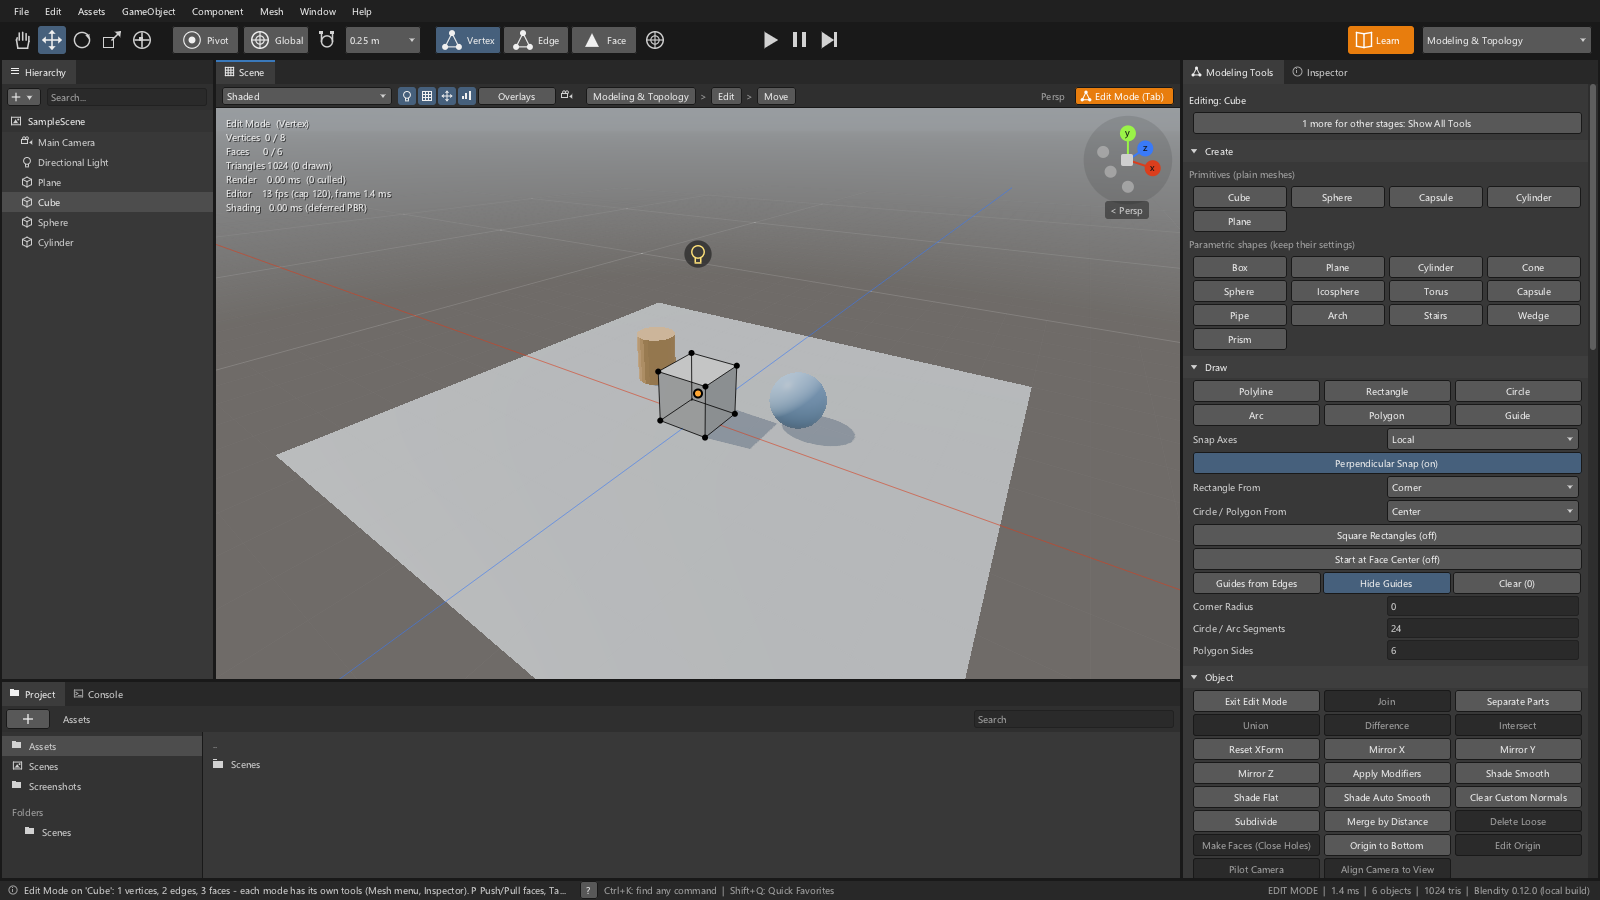
\includegraphics[width=\textwidth, alt={The Modeling and Topology layout with a cube in Edit Mode: the Scene view with the cube's cage and the Edit Mode bar, the Modeling Tools window listing the Select, Create and Extrude, Cut and Divide and Merge and Clean Up sections, the Draw tools and the checks.}]{layout-modeling.png}
  \caption{The Modeling \& Topology layout in Edit Mode: the Modeling Tools window shows the Edit Mode sections (Select,
  Create \& Extrude, Cut \& Divide, Merge \& Clean Up), the Draw tools and the checks.}
\end{figure}

\section{Navigating}
With Unity's mouse (the default feel): \key{Alt}+left drag orbits, middle drag pans, the wheel zooms, hold the right
button and use \key{W A S D} (\key{Q} / \key{E} down and up, \key{Shift} faster) to fly, \key{F} frames the selection. Click
the cones of the gizmo in the corner for front, top and side views, its centre for perspective or orthographic.
\menu{Edit > Editor Feel} switches the mouse navigation and the keys together to Unreal's, Blender's or Maya's
(chapter~\ref{ch:comingfrom}).

\section{Selecting and moving}
Click to select, \key{Ctrl}+click to add, drag a box. \key{Q W E R Y} pick the View, Move, Rotate, Scale and Transform
tools; Blender's \key{G} / \key{R} / \key{S} also work, with \key{X} / \key{Y} / \key{Z} to lock an axis and a typed number
(the Blender keys for R and S are a preference, since R is Unity's Scale tool). Hold \key{Ctrl} to snap (the increment is
the dropdown beside the magnet); \key{Ctrl+Shift} while moving drops the object onto the surface under the mouse;
\key{V} snaps a vertex onto another. While dragging a gizmo arrow, type a number to move exactly that far.

\section{Objects, components and the Inspector}
As in Unity, everything in a scene is a GameObject with a Transform; what it does comes from its components
(MeshFilter, MeshRenderer, Light, Camera, Rigidbody, Animation, modifiers, Camera Filters, \ldots). Create objects from
the Hierarchy's right-click menu or the \menu{GameObject} menu; drag a Hierarchy row onto another to parent it (in
thirds: above, into, below). The Inspector shows each component's first seven fields and keeps the rest under
\ui{Show more}; \ui{All Fields} shows everything. Number fields take expressions: \code{2*pi}, \code{+=1}, \code{*=2}
(relative to each object's own value), \code{L(0,10)} (spread evenly across the selection), \code{R(0,1)} (random per
object); with several objects selected a change applies to all of them. A field that names another object takes a typed
name or a row dragged from the Hierarchy; an asset field takes a file dragged from the Project window. Right-click a
field's name for \ui{Reset to Default} or \ui{Insert Keyframe}.

\section{Origins, Play, undo}
\menu{GameObject > Set Origin} moves the pivot to the bounds centre, the median, the centre of mass, the bottom centre,
a point, the edit selection or the view pivot without moving anything on screen; \ui{Edit Origin (Handles)} moves only
the origin with the gizmo and snaps it to vertices, edges and faces. \key{Ctrl+P} plays the scene; changes made while
playing are thrown away on Stop, as in Unity. \key{Ctrl+Z} / \key{Ctrl+Y} undo and redo the scene, materials, textures
and clips as one step per operation; \menu{Window > History} lists every step and a click goes back to it.

\section{Finding anything: the palette, favorites, the Wheel}
\key{Ctrl+K} (or \key{F3}, Blender's key) opens the \textbf{command palette}: type a few words and every action, window,
layout, creatable object and console command that matches is listed with its shortcut; \key{Enter} runs it, even a tool
the current layout hides. Right-click a row (or any menu row) for its small menu: \textbf{Quick Favorites} (\key{Shift+Q},
one list per layout), \textbf{the Wheel} (\key{Space}: one radial menu for where the mouse is, with a set per mode you
fill from any menu), \textbf{My Tools} (a window of your own panels, each a grid of commands), \textbf{Assign
Shortcut\ldots} (the next key you press binds it). Preferences $>$ UI file saves the whole arrangement (layout, windows,
feel, keymap and your shortcuts, panels, the Wheel's sets, favorites, theme, scale) as one \code{.blendity-ui} file.

\section{The status bar, toasts and the job tray}
The status bar says what the mouse and keys do where the mouse is and offers Undo for the last action; the \ui{?}
beside the hint opens the Learn lesson for what you are doing. A warning is a toast over the Scene view for three
seconds, with a \ui{Fix} button when a command puts it right (stop Play, cancel the job, unwrap first); a button that
cannot work now is dim and its tooltip says why. A long job (a bake, a remesh, a render, an export) shows in the status
bar's right slot with its progress, the time run, an estimate left and \ui{Cancel}; a toast says when it ends. The
results of checks (UV Report, Scene Statistics, Motion Check) open in a \ui{Report} dialog.

\section{Windows on other screens and Tablet Mode}
Drag any tab out past the editor's edge for a window of its own where you let go; right-click a tab for \ui{Move to New
Window}, \ui{Move to Display N} or \ui{Move to Main Window}. A Render or Game tab in its own window can be \ui{Render
Only} and \ui{Full Screen}: a second monitor showing the render large. The Scene view, the Game view and the Inspector
can be \ui{duplicated} into a new window; a second Inspector has a \ui{Pin} that keeps one object while the selection
moves on. \textbf{Tablet Mode} (the tab menu, or Preferences $>$ Pen and touch: Auto turns it on when a 2-in-1's
keyboard folds away) makes the targets half as big again, and then fingers navigate (one orbits, two pinch, pan and
twist) while the pen selects, moves, draws and paints (chapter~\ref{ch:pen}).

\section{Themes}
Preferences $>$ Theme: Dark, Light, Emiliano Light, Emiliano Dark (the palette of the author's site: paper, charcoal
and an amber accent) and High Contrast (white on near-black with every text at WCAG's 4.5:1 or more
\cite{W3C2018Web} and a yellow focus ring; the tests measure every theme's ratios).

\begin{fromnote}{Learn}
\emph{The Editor Layout}, \emph{Navigating the Scene View}, \emph{GameObjects, Components and Objects},
\emph{Hierarchy, Parenting and the Scene Graph}, \emph{Move, Rotate, Scale}, \emph{Customizing the Editor},
\emph{Undo, Selection and Memory}.
\end{fromnote}
